% ICASSP 2027 submission draft. Official Paper Kit: spconf.sty.
\documentclass{article}
\usepackage{spconf,amsmath,amssymb,graphicx,booktabs}
\usepackage[hidelinks]{hyperref}
\usepackage{array}
\usepackage{ragged2e}
\def\qmemory{policy-class Q-memory}
\def\minigrid{\textsc{MiniGrid}}
\def\qwen{Qwen2.5}
\title{Decision-Preserving Discrete Memory via Policy-Class Q-Distortion}
% ICASSP 2027 is not double-blind; list the authors and affiliations in the PDF.
\twoauthors
  {Yujie Shen}
  {School of Mathematics\\Hunan University, China\\\texttt{eugeneshen2005@gmail.com}\\\href{https://orcid.org/0009-0009-0447-9913}{ORCID: 0009-0009-0447-9913}}
  {Haowen Chen\sthanks{Corresponding author: \texttt{hwchen@hnu.edu.cn}.}}
  {College of Computer Science\\and Electronic Engineering\\Hunan University, China\\\texttt{hwchen@hnu.edu.cn}\\\href{https://orcid.org/0000-0002-4777-7525}{ORCID: 0000-0002-4777-7525}}
\renewcommand{\arraystretch}{1.08}
\setlength{\tabcolsep}{3.5pt}
\newcommand{\tabhead}[1]{\textbf{#1}}

\begin{document}
\ninept
\maketitle

\begin{abstract}
History compression for sequential decisions is usually trained with text reconstruction or a scalar task reward, neither of which specifies which distinctions must survive for action selection. We define policy-class Q-memory: a rate-constrained discrete state trained to preserve centered action advantages for a declared reference-policy class and candidate-action set. Counterfactual replay supplies the targets without simulator state at deployment. On action-ambiguous language tasks, two codes reach 100\% held-out accuracy, while one-code and text/reward controls remain at chance. A frozen \qwen-3B interface preserves 150/150 decisions with learned compressed state, matching full history. In non-oracle \minigrid{} Memory, four-code Q-memory reaches 99.76\% on S13 Random and 98.04\% on the longer S17 Random, near a continuous recurrent state and far above short-window and reconstruction controls. A 2,000-episode replay audit gives exact agreement with explicit policy classes. The evidence supports a bounded, policy-relative mechanism claim, not universal state sufficiency or open-ended-agent improvement.
\end{abstract}
\begin{keywords}
Memory compression, value-aware representation, partially observable control, rate--distortion, language agents
\end{keywords}

\section{Introduction}
Long-horizon systems must compress histories containing observations, actions, feedback, and language. The relevant question is not whether a summary reconstructs the history, but whether it preserves distinctions that change a later action. Text reconstruction can spend capacity on nondiscriminative detail; a small cue can instead reverse the best action while leaving most of the history unchanged.

Value-aware abstraction provides a decision-relative alternative. DeepMDP and value-equivalence methods preserve reward- and Bellman-relevant structure \cite{gelada2019deepmdp,grimm2020value}; prompt-compression work makes rate and distortion explicit \cite{zhu2025turbo,nagle2024limits}. We operationalize this idea for recurrent language histories by declaring (i) a finite reference policy class, (ii) covered candidate actions, and (iii) a replay protocol that estimates each action's value from a history-consistent snapshot. The resulting code is evaluated only for that declared interface.

Our contributions are: a policy-class Q-distortion objective for low-rate discrete recurrent memory; an action-ambiguous language benchmark that removes action-name shortcuts; transfer to a public partially observable \minigrid{} Memory task with standard actions; and an audit showing that replay-derived labels reproduce explicit policy-class results. We deliberately exclude open-ended agent claims.

\begin{figure*}[t]
\centering
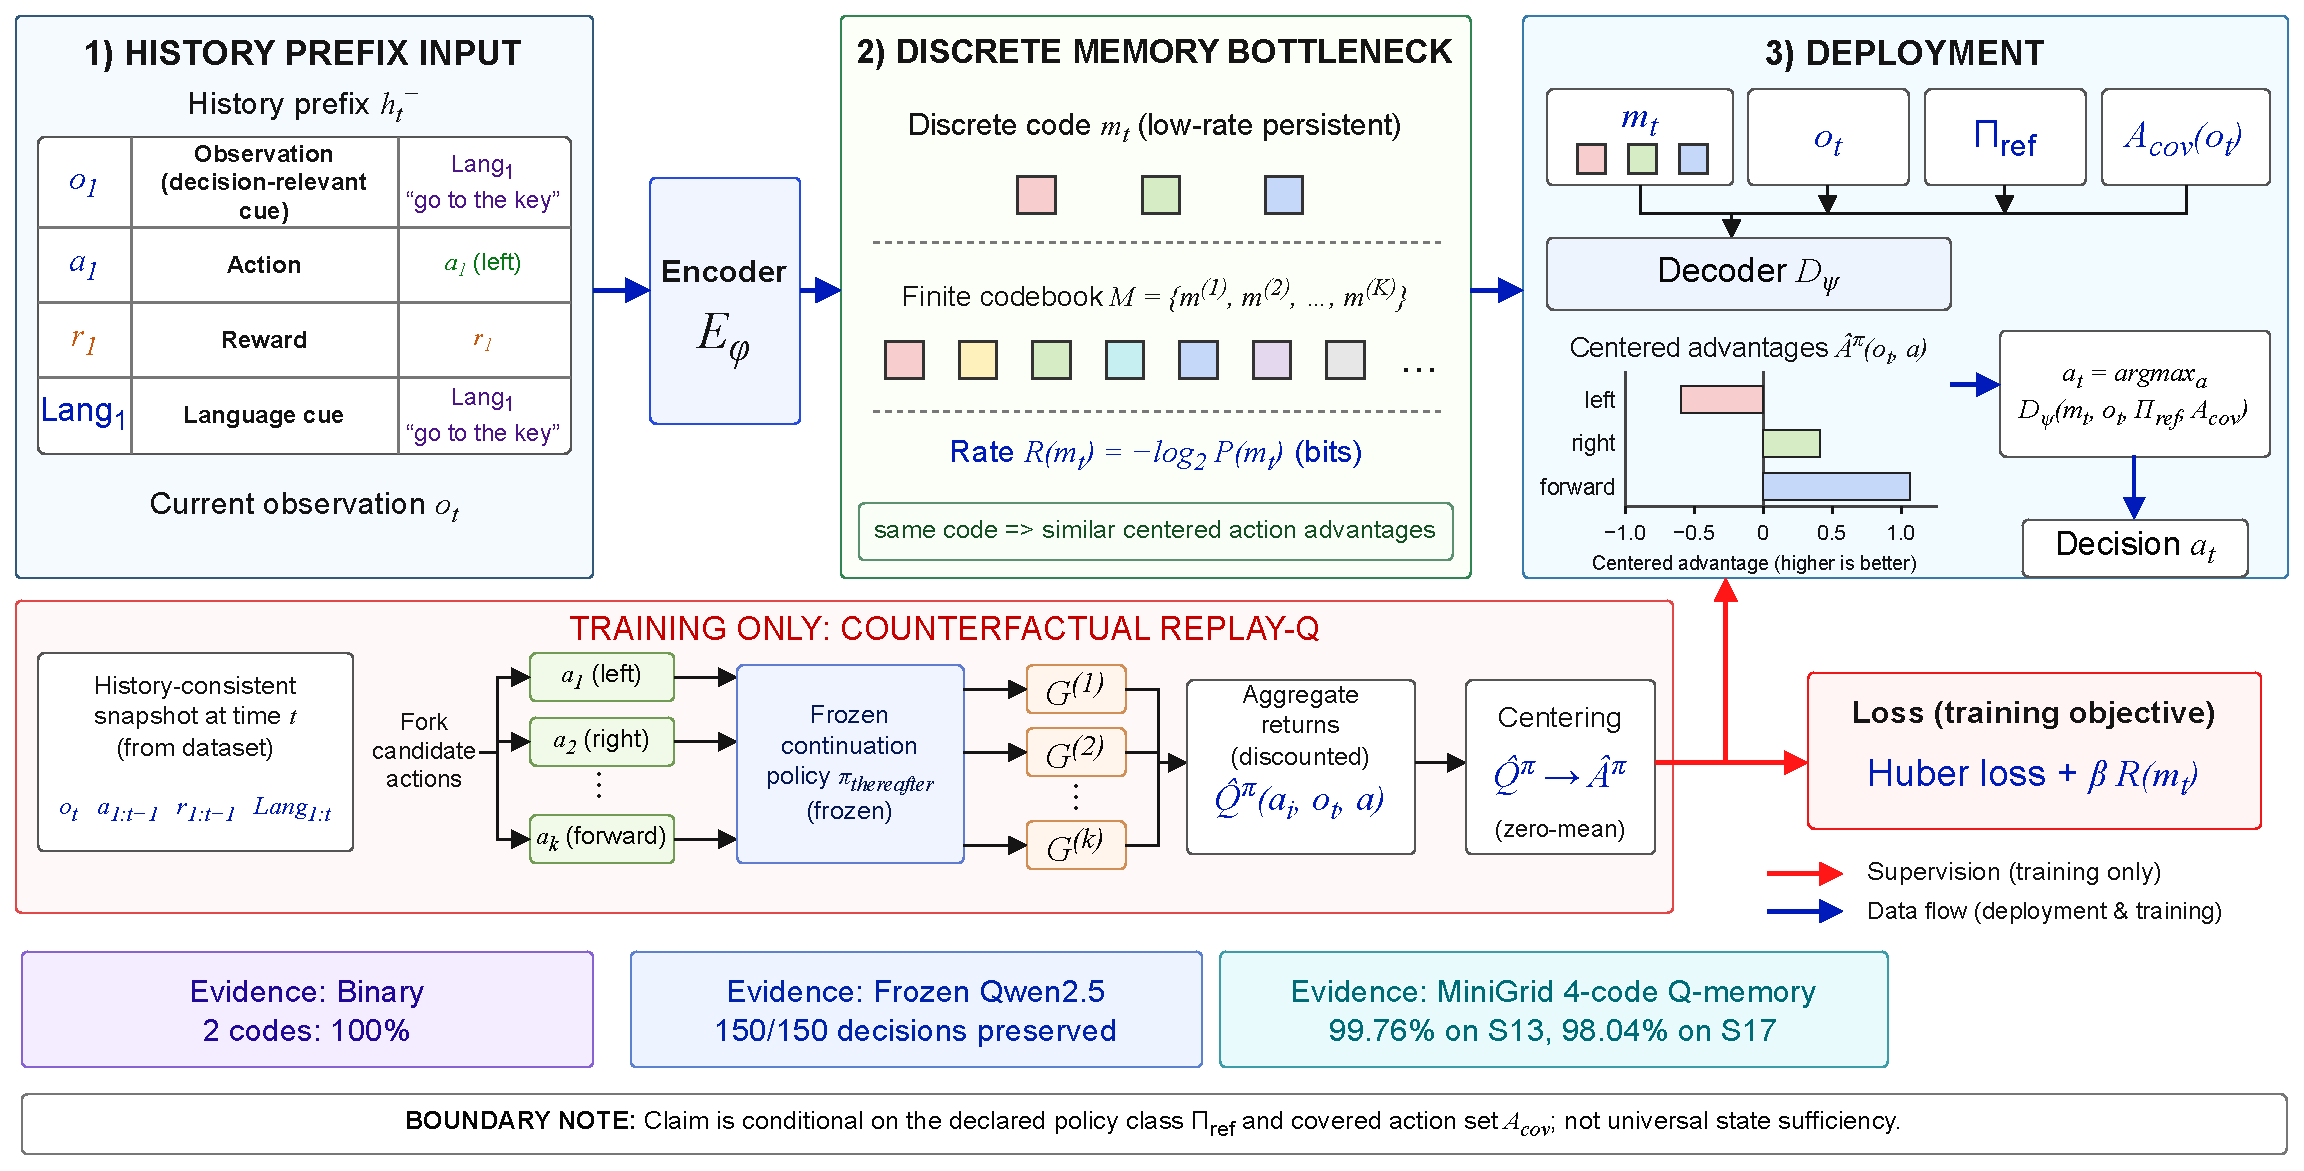
\includegraphics[width=0.77\textwidth]{policy_class_q_memory_main_figure.pdf}
\caption{Overview of policy-class Q-memory. The history prefix is encoded into a low-rate discrete code. Counterfactual replay is used during training only; deployment uses the code, current observation, declared policy class, and covered actions to select the largest decoded advantage. Bottom panels summarize the three primary evidence settings.}
\label{fig:overview}
\end{figure*}

\section{Related Work}
\textbf{Value-aware abstraction.} Representation learning for partially observable control has repeatedly separated task-relevant information from input reconstruction. POMDP planning formalizes the need to retain information that changes future decisions \cite{kaelbling1998planning,puterman1994mdp}; state-abstraction work studies homomorphisms, bisimulation metrics, and value-preserving partitions \cite{li2006unified,ferns2004metrics,abel2016state}. DeepMDP constrains a latent model using rewards and transitions, while the value-equivalence principle characterizes abstractions that preserve Bellman-relevant updates \cite{gelada2019deepmdp,grimm2020value}. Q-memory follows this decision-relative perspective but changes the object being compressed: its input is a recurrent language or observation history, its output is a low-rate discrete symbol, and its target is an action-advantage vector rather than a latent transition model. The reference policy class is explicit, so the abstraction is intentionally conditional rather than universal.

\textbf{Memory and prompt compression.} Recurrent value-based agents demonstrate that learned memory can recover information hidden by partial observability \cite{hausknecht2015deep,kapturowski2019recurrent}; representation-learning methods such as CURL show that a compact state can also be trained without reconstructing every input detail \cite{laskin2020curl}. Recent agent-memory systems store workflows, linked memories, reasoning traces, or learned compact states \cite{wang2025awm,xu2025amem,ouyang2026reasoningbank,zhou2026mem1,wu2025longmemeval}. Prompt-compression studies make rate and distortion explicit for language-model interfaces \cite{zhu2025turbo,nagle2024limits}. These methods optimize different notions of fidelity: text reconstruction preserves observations, retrieval preserves similarity to stored episodes, and scalar reward prediction preserves an outcome average. Q-memory instead preserves contrasts between covered actions under a declared downstream policy family.

\textbf{Scope.} The contribution is an implementable bridge between value-aware abstraction and sequential history compression. Counterfactual replay supplies action-conditioned targets; a discrete bottleneck makes the rate explicit; and evaluation uses action-ambiguous language plus a public non-oracle control interface. We do not claim a general-purpose language-agent architecture, universal state sufficiency, or superiority on open-ended benchmarks.

\section{Method}
Let $h_t^-$ denote the interaction prefix before the current observation $o_t$. An encoder produces a persistent code $m_t=E_\phi(h_t^-)$ with rate $R(m_t)$. For a finite class $\Pi_{\rm ref}$ and covered set $A_{\rm cov}(o_t)$, replay estimates
\begin{equation}
\widehat Q^\pi(h_t^-,o_t,a)=\widehat{\mathbb E}[G_t\mid h_t^-,o_t,a_t=a,\pi\ \text{thereafter}].
\end{equation}
We train on centered advantages
\begin{equation}
\widehat A^\pi(h_t^-,o_t,a)=\widehat Q^\pi(h_t^-,o_t,a)-|A_{\rm cov}|^{-1}\sum_b\widehat Q^\pi(h_t^-,o_t,b),
\end{equation}
which remove history-specific return offsets while retaining action rankings. The policy-class distortion is
\begin{equation}
d_Q(h,h'\mid o)=\max_{\pi\in\Pi_{\rm ref},a\in A_{\rm cov}}|A^\pi(h,o,a)-A^\pi(h',o,a)|.
\end{equation}
A code is $\epsilon$-Q-sufficient on the evaluated support when same-code histories have distortion at most $\epsilon$; this is conditional on the class and action coverage.

\subsection{Replay-Q construction}
For each training prefix, we reset or replay the environment to the snapshot defined by its observed action prefix and current observation. Every covered candidate action is executed from that identical snapshot, using paired random seeds where stochasticity is present. A frozen continuation policy supplies subsequent actions until the fixed horizon. Branch returns are aggregated to obtain $\widehat Q$ using the standard discounted-return convention \cite{sutton2018rl}, and the centered vector becomes the target for the code. The memory encoder never receives coordinates, hidden object identities, privileged admissible-action lists, or future observations.

The protocol separates three leakage channels. Train and test splits are made by base episode, world seed, and language template before branching. Future observations are excluded from both the encoded prefix and label input. Replay is accepted only when the snapshot is history-consistent; otherwise a branch value can silently become a privileged latent-state value. The reported \minigrid{} audit checks this condition by comparing replay-derived anonymous classes with explicit policy-equivalence classes.

The decoder $D_\psi(m,o,\pi,a)$ is trained with a Huber loss and rate penalty,
\begin{equation}
\mathcal L=\mathbb E\left[w\rho(D_\psi(E_\phi(h),o,\pi,a)-\widehat A^\pi)\right]+\beta\mathbb E[R(E_\phi(h))],
\end{equation}
where $w$ is a clipped inverse-variance replay weight. At deployment, only $(m,o,\pi,A_{\rm cov})$ is available. Replay uses paired candidate branches and fixed continuation policies; the encoder sees no coordinates, object identities, or future observations. A uniform decoder error $\epsilon_M$ and replay error $\epsilon_Q$ give covered-action one-step regret at most $2(\epsilon_M+\epsilon_Q)$ under simultaneous error control.

In the controlled language tasks, the encoder is a recurrent or positional-attention network followed by a learned codebook. A code is serialized as a short symbol sequence and can be passed to a frozen language-model interface. In \minigrid{}, the encoder receives the standard partial observation and action/reward history; the policy receives the code and current observation only. Codebook size is varied independently of decoder width, separating capacity from supervision. The objective is invariant to adding a history-dependent constant to all candidate values, but changes when one candidate's value changes; this is the intended decision-relative distortion.

\subsection{Controls and evaluation contract}
Every comparison uses the same current-observation interface, candidate action names, split, and evaluation seeds. Controls include one-code memory, a recent observation window, current-observation reconstruction, ordered-text reconstruction, scalar reward prediction, policy-only discrete training, continuous recurrent state, and learned full-history retrieval. The primary language task uses symmetric action strings, while the primary \minigrid{} test exposes only \texttt{left/right/forward}; neither evaluation gives the encoder a privileged action list.

\section{Experiments}
All comparisons use matched splits, candidate names, code capacity, and seeds. Language experiments average five seeds. The binary task has two symmetric action strings and a delayed cue; the natural-language task adds paraphrases, distractors, and held-out templates (6,000 train/2,000 test). A four-state extension uses 8,000/3,000 examples. The frozen \qwen{} experiment evaluates 150 held-out episodes. \minigrid{} uses version 2.3.1, standard 7$\times$7 partial observations, actions \texttt{left/right/forward}, 2,000 trajectories per training seed, five seeds, and 500 shared held-out world seeds. Training uses Python/PyTorch on one RTX 4090; \minigrid{} itself does not require an LLM.

\subsection{Controlled language benchmarks}
The binary benchmark contains an early cue, intervening state updates, distractor descriptions, and a final decision between two identical action strings. The cue is not repeated at the decision point, so the action name cannot reveal the answer. We generate independent training and test episodes and evaluate each seed on 2,000 held-out episodes. The natural-language version replaces symbolic states with paraphrased descriptions, inserts irrelevant clauses, and holds out paraphrase templates. Its Q target, ordered-text reconstruction, and scalar-reward conditions use the same positional-attention encoder, two-code bottleneck, split, and optimizer budget. The four-state extension tests scaling beyond a binary partition using four action classes and unseen language templates.

\subsection{Frozen language-model interface}
To test whether the code is usable by a downstream model without fine-tuning that model, we freeze a \qwen-3B decision interface. Each held-out episode is evaluated under full history, learned compressed state, and a truncated final segment. The interface receives the same current observation and candidate actions in all conditions. This is a retention test: a tie between full history and compressed state supports preservation of the reference decision, not an improvement claim.

\subsection{Non-oracle partially observable control}
We use \texttt{MiniGrid-MemoryS13Random-v0} as the primary mechanism task and evaluate zero-shot on S11 and the longer S17 Random variants. The policy sees a standard 7$\times$7 partial observation and chooses only \texttt{left}, \texttt{right}, or \texttt{forward}. Five independently initialized models are trained from 2,000 trajectories per seed. All methods are evaluated on the same 500 held-out world seeds. An independent expert audit solves all held-out seeds and checks cue balance, so a low control score cannot be attributed to failed environments or a missing class.

\begin{table}[t]
\centering
\caption{Controlled language and frozen-backbone evidence. Mean $\pm$ seed SD where applicable.}
\label{tab:controlled}
\begin{tabular}{@{}>{\raggedright\arraybackslash}p{.57\columnwidth}>{\raggedright\arraybackslash}p{.34\columnwidth}@{}}
\toprule
Experiment / condition & Result\\
\midrule
Binary, one code & 50.10 $\pm$ 0.42\%\\
Binary, two codes & \textbf{100.00\%}\\
Binary, four / eight codes & 99.97 $\pm$ 0.06 / 0.04\%\\
Natural language, Q target & \textbf{98.47 $\pm$ 3.06\%}\\
Natural language, text reconstruction & 51.11 $\pm$ 3.24\%\\
Natural language, scalar reward & 29.81 $\pm$ 18.31\%\\
Four-state, four-way code (5 seeds) & 100\% train and test\\
Frozen \qwen{} (full / compressed / truncated) & 150/150; 150/150; 68/150\\
\bottomrule
\end{tabular}
\end{table}

The two-code result isolates the mechanism: one code cannot separate the two policy classes, whereas sufficient capacity preserves the delayed decision. With the same encoder and bottleneck, Q supervision succeeds while text reconstruction and scalar reward prediction do not. The four-state extension reaches 100\% across all five seeds. A frozen \qwen-3B decision interface makes the compressed code operational: it preserves every decision made from full history, while truncation loses more than half.

The objective comparison is informative because all three learned conditions have the same nominal rate. Ordered reconstruction models the full sequence, but its loss weights distractor tokens and does not force the two decision classes apart. Scalar reward prediction collapses action-conditioned contrasts into one number. Q supervision presents the decoder with the vector needed to rank covered actions, which is why the result survives the symmetric-action construction.

\begin{table}[t]
\centering
\caption{Non-oracle \minigrid{} Memory performance (mean $\pm$ seed SD, percent).}
\label{tab:minigrid}
\setlength{\tabcolsep}{1.8pt}
\begin{tabular}{@{}>{\raggedright\arraybackslash}p{.28\columnwidth}>{\centering\arraybackslash}p{.225\columnwidth}>{\centering\arraybackslash}p{.225\columnwidth}>{\centering\arraybackslash}p{.225\columnwidth}@{}}
\toprule
Model & S13 & S11 & S17\\
\midrule
Q-memory (4 codes) & \textbf{99.76 $\pm$ 0.54} & \textbf{100.00 $\pm$ 0.00} & \textbf{98.04 $\pm$ 2.63}\\
Continuous recurrent & 100.00 $\pm$ 0.00 & 100.00 $\pm$ 0.00 & 100.00 $\pm$ 0.00\\
Full-history retrieval & 85.12 $\pm$ 22.23 & 86.36 $\pm$ 21.38 & 85.88 $\pm$ 21.86\\
Q-memory (1 code) & 51.80 $\pm$ 2.68 & 49.76 $\pm$ 0.36 & 51.80 $\pm$ 2.68\\
Recent window (4) & 50.60 $\pm$ 3.29 & 49.92 $\pm$ 0.44 & 50.60 $\pm$ 3.29\\
Observation reconstruction & 49.40 $\pm$ 3.29 & 50.08 $\pm$ 0.44 & 49.40 $\pm$ 3.29\\
Policy-only discrete & 50.60 $\pm$ 3.29 & 49.92 $\pm$ 0.44 & 50.60 $\pm$ 3.29\\
\bottomrule
\end{tabular}
\end{table}

On S13, Q-memory exceeds one-code, recent-window, reconstruction, and policy-only controls by 47.96, 49.16, 50.36, and 49.16 points, respectively, and is within 0.24 points of the continuous state. Retrieval is useful but seed-unstable (one seed 46.6\%); we do not claim universal retrieval superiority. The longer S17 result remains above 98\% but has larger seed variation.

The S11 and S17 transfer tests probe two risks. S11 is shorter and checks whether the same policy partition transfers across a changed random layout. S17 adds a longer delay and stresses propagation of the decision-relevant class. Performance remains high on both, but the larger S17 seed deviation argues against treating the discrete optimizer as failure-free. The continuous state reaches the ceiling on all three variants and serves as a capacity reference rather than a compression baseline.

\begin{table}[t]
\centering
\caption{Capacity, data, and replay-Q audit. Values are mean $\pm$ seed SD unless exact.}
\label{tab:audit}
\setlength{\tabcolsep}{2.8pt}
\begin{tabular}{@{}>{\raggedright\arraybackslash}p{.30\columnwidth}>{\raggedright\arraybackslash}p{.58\columnwidth}@{}}
\toprule
Audit & Result\\
\midrule
Capacity & 1 code: 51.80 $\pm$ 2.68\%; 3: 90.12 $\pm$ 13.60\%; 4: \textbf{99.76 $\pm$ 0.54\%}; 8: 99.76 $\pm$ 0.54\%\\
Training data & 250: 46.24 $\pm$ 20.14\%; 500: 89.72 $\pm$ 22.54\%; 1,000: 99.36 $\pm$ 0.61\%; 2,000: 99.04 $\pm$ 0.78\%\\
Replay labels & 2,000/2,000 agree; class counts 1,002/998\\
Paired trajectories & 7,500/7,500 outcomes, actions, and codes identical\\
Sparse target controls & 47.0\%; 47.2\%\\
\bottomrule
\end{tabular}
\end{table}

The capacity sweep shows an optimization threshold: three codes are theoretically sufficient but unstable, while four are reliable. Replay-derived labels reproduce explicit labels exactly under matched seeds, closing the objection that semantic class names drive the result. However, sparse downstream action targets alone remain at chance; the method requires structured replay-Q supervision rather than a single terminal reward.

The nested data sweep separates representational capacity from optimization reliability. Four-code Q-memory is near ceiling with 1,000 trajectories, whereas 250 examples are insufficient despite the same nominal code size. The plateau from 1,000 to 2,000 suggests that the main bottleneck is learning the temporal partition, not increasing codebook size. These values are protocol-specific sample-efficiency measurements rather than a universal data requirement.

\subsection{Replay audit and negative controls}
The final audit removes human-readable class names. Anonymous classes are recovered from counterfactual branch rewards and the successful terminal standard observation, then propagated through the same training pipeline. Replay labels agree with explicit policy-equivalence classes on all 2,000 audited episodes, and paired models produce identical outcomes, action sequences, and codes on all 7,500 comparisons. Two additional models trained only on sparse downstream action targets remain near chance. Semantic names are therefore unnecessary, but structured counterfactual supervision remains essential.

\section{Discussion and limitations}
Across controlled language and non-oracle partial observation, a small discrete state preserves delayed decisions when trained on action-conditioned differences. The comparison controls show that the gain is not a generic bottleneck effect. Centered advantages retain the information needed to compare covered actions and discard offsets irrelevant to choice. The replay audit shows that semantic names are unnecessary, but replay branches, expert continuations, and temporal propagation remain supervision and can be expensive.

The claim is relative to the frozen policy class, candidate coverage, history-consistent snapshots, and evaluated support. A changed policy may need discarded distinctions; inadequate coverage or replay uncertainty can invalidate the target. Results do not establish universal state sufficiency, automatic discovery from sparse reward, or improvement on open-ended agent benchmarks. Reproducibility requires releasing generators, split manifests, seeds, checkpoints, environment lockfiles, and scripts for every table.

There is an offline-cost trade-off. Counterfactual branching multiplies environment interaction during target construction, whereas deployment uses only a compact code and the current observation. Whether this exchange is beneficial depends on episode length, branch count, and how often the reference policy class changes. A practical deployment would cache replay targets, report coverage and uncertainty, and retrain when the candidate interface changes. The current study measures decision preservation under a fixed interface, not wall-clock savings in a production agent.

\section{Conclusion}
Policy-class Q-memory defines a narrow, testable notion of sufficient memory: histories that share a code should induce similar centered action advantages for a declared policy family and covered action set. Across action-ambiguous language, a frozen \qwen{} interface, and non-oracle \minigrid{}, low-rate discrete codes preserve delayed decisions when trained with replay-derived Q targets. Text reconstruction, scalar reward prediction, short windows, and sparse downstream targets fail under matched controls. The result motivates decision-relative compression as a design primitive, while universal abstractions, changing policy classes, open-ended agents, and end-to-end sparse-reward discovery remain open problems.

\section{Implementation Details}
\emergencystretch=3em
\textbf{Language generators.} The binary action-ambiguous generator samples an early cue, a sequence of state updates, distractor descriptions, and a final choice between two symmetric action strings. The cue is not repeated at the decision point. Training and test histories use disjoint episode seeds. The natural-language generator uses four training paraphrase templates and three held-out templates, with distractor clauses inserted at variable positions. The four-state extension uses four action classes and unseen templates; 8,000 examples are used for training and 3,000 for testing. All language rates average five independently initialized models.

\textbf{Memory and optimization.} The encoder consumes the prefix sequentially and emits a code from a learned finite codebook. The decoder receives the code, current observation, policy identifier, and candidate action. Q-target and control conditions use the same encoder and decoder widths, code capacity, split, and optimizer budget. For the frozen language-model interface, the selected code is serialized as a fixed short symbol string. No condition reads a future observation or environment coordinate.

\textbf{MiniGrid protocol.} We train on the S13 Random Memory environment and evaluate zero-shot on S11 and S17 Random, using MiniGrid version 2.3.1. The policy receives a standard 7$\times$7 partial observation and selects only \texttt{left}, \texttt{right}, or \texttt{forward}. Five seeds use 2,000 trajectories each; every method uses the same 500 held-out world seeds. An expert audit solves all 500 seeds; cue classes occur 246/254 on S13 and remain balanced on transfer variants.

\textbf{Statistical reporting.} Episode-level rates use 95\% Wilson intervals when intervals are reported; the tables show mean and standard deviation across training seeds to expose optimization variation. Seed variation is not counted as additional episode samples. Paired model differences use hierarchical bootstrap resampling over training seeds and paired held-out tasks. The 7,500 trajectory identity result is a matched reproducibility audit, not 7,500 independent environments. The frozen \qwen{} comparison is a retention test over a shared generated task family, not a general language-agent claim.

\textbf{Reproducibility and availability.} Code and reported artifacts are available at \url{https://github.com/JJayshum/Q-Memory}. The repository contains synthetic-task generators, MiniGrid and language-task results, replay-Q audit files, capacity and data sweeps, and statistical summaries. It does not yet include all environment lockfiles, generated split manifests, or model checkpoints; these are required for a complete archival release. Third-party model weights should be referenced through their official distribution mechanism.

\section{Acknowledgment}
This work was supported by the National Natural Science Foundation of China (grant no.~62472165), the Fundamental and Interdisciplinary Disciplines Breakthrough Plan of the Ministry of Education of China (JYB2025XDXM602), and the Yuelushan Laboratory Breeding Program (YLS-2026-ZY01002).

\begin{thebibliography}{10}
\bibitem{gelada2019deepmdp} C. Gelada, S. Kumar, J. Buckman, O. Nachum, and M. G. Bellemare, ``DeepMDP: Learning continuous latent space models for representation learning,'' in \emph{Proc. ICML}, vol. 97, pp. 2170--2179, 2019.
\bibitem{grimm2020value} C. Grimm, A. Barreto, S. Singh, and D. Silver, ``The value equivalence principle for model-based reinforcement learning,'' in \emph{Proc. NeurIPS}, vol. 33, pp. 5541--5552, 2020.
\bibitem{zhu2025turbo} X. Zhu, P. Tang, H. Liao, and S. Appalaraju, ``Turbocharging web automation: The impact of compressed history states,'' in \emph{Findings of ACL}, pp. 3644--3651, 2025.
\bibitem{nagle2024limits} A. Nagle, A. Girish, M. Bondaschi, M. Gastpar, A. V. Makkuva, and H. Kim, ``Fundamental limits of prompt compression: A rate-distortion framework for black-box language models,'' in \emph{Proc. NeurIPS}, vol. 37, pp. 94934--94970, 2024.
\bibitem{kaelbling1998planning} L. P. Kaelbling, M. L. Littman, and A. R. Cassandra, ``Planning and acting in partially observable stochastic domains,'' \emph{Artificial Intelligence}, vol. 101, no. 1--2, pp. 99--134, 1998.
\bibitem{puterman1994mdp} M. L. Puterman, \emph{Markov Decision Processes: Discrete Stochastic Dynamic Programming}. Wiley, 1994.
\bibitem{li2006unified} L. Li, T. J. Walsh, and M. L. Littman, ``Towards a unified theory of state abstraction for MDPs,'' in \emph{Proc. Ninth Int. Symp. Artificial Intelligence and Mathematics}, 2006.
\bibitem{ferns2004metrics} N. Ferns, P. Panangaden, and R. Precup, ``Metrics for finite Markov decision processes,'' in \emph{Proc. 20th Conf. Uncertainty in Artificial Intelligence}, pp. 162--177, 2004.
\bibitem{abel2016state} D. Abel, D. Hershkowitz, and M. Littman, ``Near optimal behavior via approximate state abstraction,'' in \emph{Proc. ICML}, vol. 48, pp. 2915--2923, 2016.
\bibitem{hausknecht2015deep} M. Hausknecht and P. Stone, ``Deep recurrent Q-learning for partially observable MDPs,'' arXiv:1507.06527, 2015.
\bibitem{kapturowski2019recurrent} S. Kapturowski \emph{et al.}, ``Recurrent experience replay in distributed reinforcement learning,'' in \emph{Proc. ICLR}, 2019.
\bibitem{laskin2020curl} M. Laskin, A. Srinivas, and P. Abbeel, ``CURL: Contrastive unsupervised representations for reinforcement learning,'' in \emph{Proc. ICML}, vol. 119, pp. 5639--5650, 2020.
\bibitem{wang2025awm} Z. Z. Wang, J. Mao, D. Fried, and G. Neubig, ``Agent workflow memory,'' in \emph{Proc. ICML}, vol. 267, pp. 63897--63911, 2025.
\bibitem{xu2025amem} W. Xu \emph{et al.}, ``A-Mem: Agentic memory for LLM agents,'' in \emph{Proc. NeurIPS}, vol. 38, pp. 20004--20031, 2025.
\bibitem{ouyang2026reasoningbank} S. Ouyang \emph{et al.}, ``ReasoningBank: Scaling agent self-evolving with reasoning memory,'' in \emph{Proc. ICLR}, 2026.
\bibitem{zhou2026mem1} Z. Zhou \emph{et al.}, ``MEM1: Learning to synergize memory and reasoning for efficient long-horizon agents,'' arXiv:2506.15841, 2025.
\bibitem{wu2025longmemeval} D. Wu \emph{et al.}, ``LongMemEval: Benchmarking chat assistants on long-term interactive memory,'' in \emph{Proc. ICLR}, 2025.
\bibitem{sutton2018rl} R. S. Sutton and A. G. Barto, \emph{Reinforcement Learning: An Introduction}, 2nd ed. MIT Press, 2018.
\end{thebibliography}
\end{document}
